\documentclass[12pt, a4paper, twoside]{article}
\usepackage{../labreport}
\usepackage{pdfpages}
\usepackage{circuitikz}
\usepackage{adjustbox}

\setlabreportopts[authors={Nandor Kovacs \& Céline Schuster},
    title={Glühlämpchen},
    subtitle={Aufbau von einfachen Schaltkreisen, und die Messung von Strom und Spannung},
    date={\today},
    labdate={24. März 2022}
]

\pgfplotsset{compat=1.16}
\begin{document}
\maketitlepage
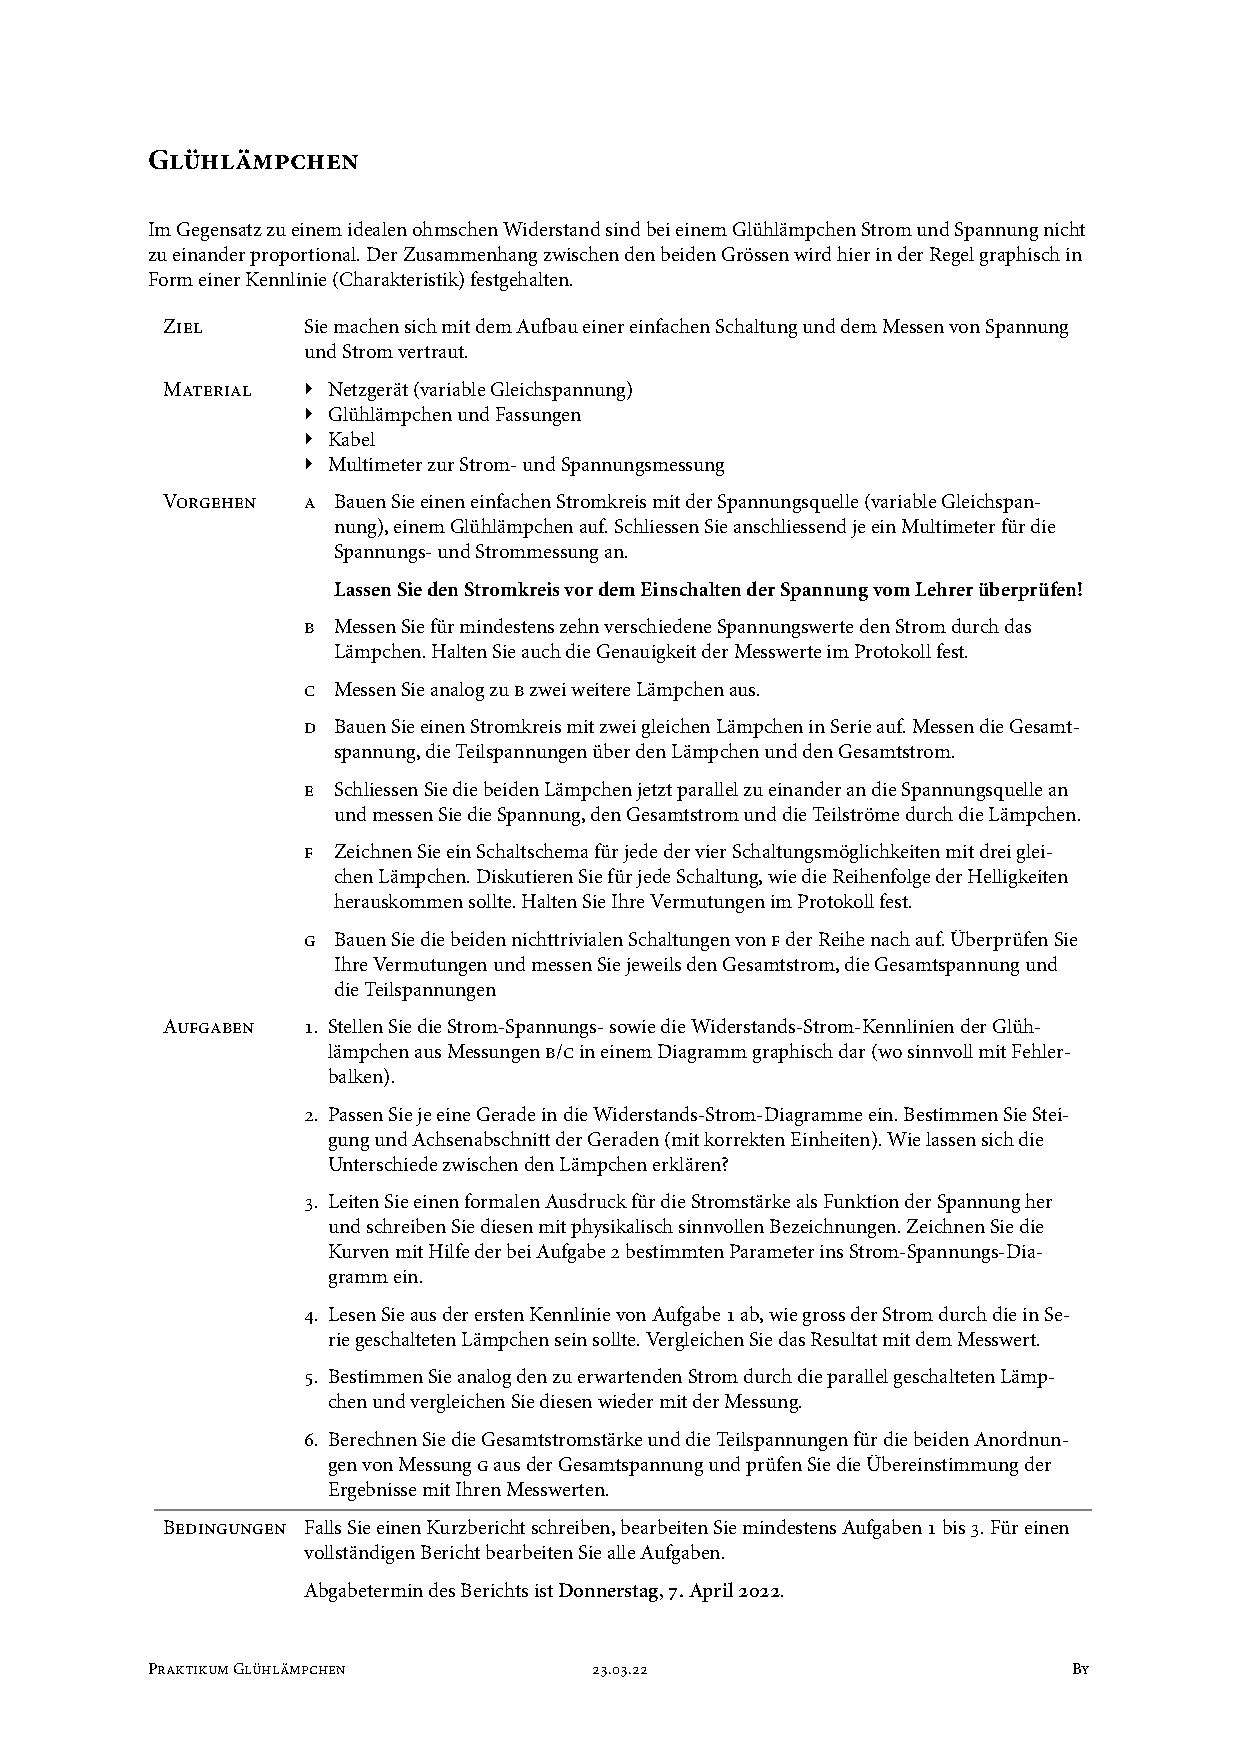
\includepdf[pages={1}]{aufgabenstellung.pdf}
\section{Einleitung}
Im Gegensatz zu herkömmlichen Widerständen ($R$) sind Strom ($I$) und Spannung ($U$) bei Glühlampen nicht proportional zueinander. Dennoch stehen diese Größen in einem gewissen Verhältnis.
In diesem Praktikum messen wir alle Werte in verschiedenen Szenarien, um ihre Beziehung herauszufinden.


\section{Theorie}
Alle unsere Schaltkreise haben drei Hauptparameter:
\begin{list}{-}{}
  \item $I$ = die Stromspannung
  \item $U$ = die Stromstärke
\end{list}

\section{Experiment}
Das Experiment bestand aus verschiedenen Stromkreisen, und Messungen an diesen Stromkreisen.
\par
Für dem folgenden Stromkreis haben wir zehn Messungen gemacht für das Lämpchen 1, 5 für Lämpchen 2, und weitere 5 für Lämpchen 3.
Bei allen zehn haben wir verschiedene Spannungen angehängt.\\

\circuit{
  (0, 0) to[vsource] (0, 5) to[lamp] (8, 5) to[rmeterwa, t=A, l=$I_{gemessen}$] (8, 0) -- (0, 0)
  (2, 5) -- (2, 6) to[rmeterwa, t=V, l=$U_{gemessen}$] (6, 6) -- (6, 5)

}

\datatable{c|c|c}{\csvcoli & \csvcolii & \csvcoliii}{Lämpchen 1}{$U_{start}$ & $U_{gemessen}$ & $I_{gemessen}$}{a_lamp1.csv}{a_lamp1}
\datatable{c|c|c}{\csvcoli & \csvcolii & \csvcoliii}{Lämpchen 2}{$U_{start}$ & $U_{gemessen}$ & $I_{gemessen}$}{a_lamp2.csv}{a_lamp2}
\datatable{c|c|c}{\csvcoli & \csvcolii & \csvcoliii}{Lämpchen 3}{$U_{start}$ & $U_{gemessen}$ & $I_{gemessen}$}{a_lamp2.csv}{a_lamp3}

Für diese nächsten zwei Stromkreise haben wir je eine Messung gemacht:

\circuit{
  (0, 0) to[vsource] (0, 5) to[lamp, l=1] (4, 5) to[lamp, l=2] (8, 5) to[rmeterwa, t=A, l=$I_{gemessen}$] (8, 0) -- (0, 0)
  (1, 5) -- (1, 6) to[rmeterwa, t=V, l=$U_{gemessen}$] (7, 6) -- (7, 5)
}

\datatable{c|c|c|c|c}{\csvcoli & \csvcolii & \csvcoliii & \csvcoliv & \csvcolv}{In serie geschaltet}{$U_{start}$ & $U_{gemessen}$ & $I_{total}$ & $I_{1}$ & $I_{2}$}{b_lamp1.csv}{serie}

\circuit{
  (0, 0) to[vsource] (0, 5) to[lamp, l=2] (8, 5) to[rmeterwa, t=A, l=$I_{gemessen}$] (8, 0) -- (0, 0)
  (2, 5) -- (2, 6.5) to[lamp, l=1] (6, 6.5) -- (6, 5)
  (2, 5) -- (2, 3.5) to[rmeterwa, t=V, l=$U_{gemessen}$] (6, 3.5) -- (6, 5)
}

\datatable{c|c|c|c|c}{\csvcoli & \csvcolii & \csvcoliii & \csvcoliv & \csvcolv}{Parallel geschaltet}{$U_{start}$ & $U_{gemessen}$ & $I_{total}$ & $I_{1}$ & $I_{2}$}{c_lamp1.csv}{parallel}

Bei den kommenden Diagrammen haben wir Vermutungen gestellt in Bezug auf die Lichtintensität der verschiedenen Glühlämpchen, und haben diese nacher beobachtet.
Ausserdem haben wir auch Messungen gemacht.

\circuit{
  (0, 0) to[vsource] (0, 5)
  to[lamp, l=1] (8/3, 5) to[lamp, l=2] (16/3, 5) to[lamp, l=3]
  (8, 5) -- (8, 0) -- (0, 0)
}

Vermutung: 1, 2 und 3 alle gleich hell \\
Beobachtung: Unsere Vermutung war richtig

\datatable{c|c|c|c|c|c}{\csvcoli & \csvcolii & \csvcoliii & \csvcoliv & \csvcolv & \csvcolvi}{F$i$}{$U_{start}$ & $U_{gemessen}$ & $I_{total}$ & $I_{1}$ & $I_{2}$ & $I_{3}$}{f_1.csv}{f1}

\circuit{
  (0, 0) to[vsource] (0, 5) 
  to[lamp, l=1] (4, 5) to[lamp, l=3]
  (8, 5) -- (8, 0) -- (0, 0)
  (1, 5) -- (1, 6) to[lamp, l=2] (7, 6) -- (7, 5)
}

\datatable{c|c|c|c|c|c|c}{\csvcoli & \csvcolii & \csvcoliii & \csvcoliv & \csvcolv & \csvcolvi & \csvcolvii}{F$ii$}{$U_{start}$ & $U_{gemessen}$ & $I_{total}$ & $I_{1}$ & $I_{2}$ & $I_{3}$ & $I_{1 + 3}$}{f_2.csv}{f2}

Vermutung: 1 und zwei sind gleich hell, 3 ist stärker wie 1 und 2\\
Beobachtung: Unsere Vermutung war richtig

\circuit{
  (0, 0) to[vsource] (0, 5)
  to[lamp, l=1] (3, 5) --
  (4, 5) -- (4, 6) to[lamp, l=2] (7, 6) -- (7, 5)
  (4, 5) -- (4, 4) to[lamp, l=3] (7, 4) -- (7, 5) --
  (8, 5) -- (8, 0) -- (0, 0)
}

\datatable{c|c|c|c|c|c|c}{\csvcoli & \csvcolii & \csvcoliii & \csvcoliv & \csvcolv & \csvcolvi & \csvcolvii}{F$iii$}{$U_{start}$ & $U_{gemessen}$ & $I_{total}$ & $I_{1}$ & $I_{2}$ & $I_{3}$ & $I_{2 + 3}$}{f_3.csv}{f3}

Vermutung: 1 ist am stärksten, 2 und 3 sind gleichstark.\\
Beobachtung: Unsere Vermutung war richtig


\circuit{
  (0, 0) to[vsource] (0, 5)
  to[lamp, l=2] (8, 5)
  (2, 5) -- (2, 6.5) to[lamp, l=1] (6, 6.5) -- (6, 5)
  (2, 5) -- (2, 3.5) to[lamp, l=3] (6, 3.5) -- (6, 5)
  (8, 5) -- (8, 0) -- (0, 0)
}

Hier haben wir keine Messungen gemacht \\

Vermutung: Alle sind gleichstark \\
Beobachtung: Unsere Vermutung war richtig

\section{Aufgaben}
\subsection{Strom-Spannungs- \& Wiederstands-Strom-Kennlinien}

\begin{center}
  \pgfplotsset{every axis legend/.append style={
        at={(1,0)},
        anchor=south east}}
  \begin{tikzpicture}
    \begin{axis}[
        axis lines = left,
        enlargelimits=0.2,
        ylabel={Stromstärke $I$ in Volt},
        xlabel={Spannung $U$ in milli Ampere},
        cycle list name=black white
      ]
      \addplot+[color=red] table[x expr=\thisrow{a}, y expr=\thisrow{v}, col sep=comma] {a_lamp1.csv};
      \addplot+[color=green] table[x expr=\thisrow{a}, y expr=\thisrow{v}, col sep=comma] {a_lamp2.csv};
      \addplot+[color=cyan] table[x expr=\thisrow{a}, y expr=\thisrow{v}, col sep=comma] {a_lamp3.csv};
    \end{axis}
  \end{tikzpicture}
\end{center}

\begin{center}
  \pgfplotsset{every axis legend/.append style={
        at={(1,0)},
        anchor=south east}}
  \begin{tikzpicture}
    \begin{axis}[
        axis lines = left,
        enlargelimits=0.2,
        ylabel={Widerstand $R$ in Ohm},
        xlabel={Spannung $U$ in milli Ampere},
        cycle list name=black white
      ]
      \addplot+[color=red] table[x expr=\thisrow{a}, y expr=\thisrow{v} / \thisrow{a}, col sep=comma] {a_lamp1.csv};
      \addplot+[color=green] table[x expr=\thisrow{a}, y expr=\thisrow{v} / \thisrow{a}, col sep=comma] {a_lamp2.csv};
      \addplot+[color=cyan] table[x expr=\thisrow{a}, y expr=\thisrow{v} / \thisrow{a}, col sep=comma] {a_lamp3.csv};
    \end{axis}
  \end{tikzpicture}
\end{center}

\subsection{}

\section{Fazit}
\section{Reflektion}
\section{Anhang}
Versuchsanleitung und Originalprotokoll vom \labdate
\end{document}